\chapter{Game v2: an RL project from start to finish}
\label{ch:v2-project}

On game \code{v1} the PPO agent of \cref{ch:ppo} wins about $97\%$ of the
games, and expert iteration takes it to almost $98\%$. Game \code{v2}
(\cref{sec:v2}) is much harder: a bigger maze, a ghost house, eaten ghosts
that come back, one life. This chapter follows the work on \code{v2} as it
happened, wrong turns included. The algorithms are those of the previous
chapters; what this chapter adds is method: how to measure an agent, how to
find out why it loses, and how to decide what to try next. Each lesson is
drawn out in a box, and the last section collects them.

\section{A first agent, and how to measure it}

The first agent (\emph{run 1}) is the PPO agent of \cref{ch:ppo}, trained
for $30$ million steps on a Kaggle GPU with the curriculum of the
notebooks: the ghosts' aggressiveness grows from $30\%$ to $100\%$ of its
value over the first fifth of the training. It wins no game for $8$ million
steps, and $34\%$ of its training games at the end.

That figure is not the agent's level. During the training the actions are
\emph{sampled} from the policy, so the agent sometimes plays a move it
considers worse; \code{pacman\_play.py} plays the \emph{best} action. On
$1000$ games, run 1 wins $56.3\%$ of them. How precise is that?

\begin{proposition}{Precision of a win rate}{win-rate-error}
  If an agent wins each of $n$ independent games with probability $p$, its
  observed win rate $\hat p$ has mean $p$ and standard deviation
  \begin{equation}
    \sigma(\hat p) = \sqrt{\frac{p(1 - p)}{n}} \le \frac{1}{2\sqrt n}.
  \end{equation}
  For two agents evaluated on different games, the difference of their
  rates has standard deviation $\sqrt{\sigma_1^2 + \sigma_2^2}$.
\end{proposition}

\begin{proof}
  $n \hat p$ is a sum of $n$ independent Bernoulli variables of parameter
  $p$: it has mean $np$ and variance $np(1 - p)$, and $p(1 - p) \le 1/4$.
  The variances of independent estimates add up.
\end{proof}

With $p \approx 0.6$: $1.6$ points for $1000$ games and $0.9$ for $3000$; for
the difference of two agents, $2.2$ and $1.3$ points. Differences of a few
points between agents need thousands of games.

\begin{pacman}{A lucky set of games}{lucky-games}
  A second session (\emph{run 2}) resumed run 1 for $35$ million steps at
  the final learning rate. On the same $1000$ games, run 1 won $56.3\%$ and
  run 2 $52.8\%$, so run 1 was kept. On $3000$ other games:
  \begin{center}
    \begin{tabular}{@{}lcc@{}}
      \toprule
      & $1000$ games (\code{--seed 1}) & $3000$ new games \\
      \midrule
      run 1 & $56.3\%$ & $50.1\%$ \\
      run 2 & $52.8\%$ & $50.9\%$ \\
      \bottomrule
    \end{tabular}
  \end{center}
  The first $1000$ games were a lucky draw for run 1, and choosing run 1
  \emph{on those games} made them look luckier still: among several
  agents, the one with the best score on a set of games is likely to be
  one that was lucky on it.
\end{pacman}

\begin{remark}{Lesson: evaluate on many games, and on fresh ones}{lesson-eval}
  Compare agents on thousands of games, and confirm the agent chosen as
  the best on games that played no part in the choice. From here on, each
  comparison of this chapter uses games that no earlier decision used.
\end{remark}

\begin{remark}{Lesson: the training curve is not the agent}{lesson-curve}
  Run 2 won more of its training games ($37\%$ to $42\%$) but not more of
  the evaluation games: the extra training made the sampled policy better
  without improving its best action. The training curve describes the
  policy that explores; the agent that plays is measured only by its own
  evaluation.
\end{remark}

\section{Looking at the losses}
\label{sec:v2-losses}

$95\%$ or more of the lost games are lost to the ``other'' causes of
\code{pacman\_play.py}: Pacman is caught in the middle of the game, not when
his power runs out or at the start. That is too vague to act on, so the
$1000$ games of run 1 were replayed, recording the cookies left after every
move.

\begin{pacman}{When are the games lost?}{v2-stages}
  Half of the lost games are lost with $22$ cookies left or fewer (out of
  $162$). By stage of the game:
  \begin{center}
    \begin{tabular}{@{}lccc@{}}
      \toprule
      Cookies left & Games lost there & Moves (per game) & Lost per $1000$
        moves \\
      \midrule
      $162$--$121$ & $2.9\%$ & $70$ & $0.41$ \\
      $80$--$41$ & $8.8\%$ & $83$ & $1.05$ \\
      $20$--$11$ & $8.9\%$ & $41$ & $2.19$ \\
      $5$--$1$ & $11.8\%$ & $57$ & $2.08$ \\
      \bottomrule
    \end{tabular}
  \end{center}
  Each move is $5$ to $6$ times more dangerous at the end than at the
  start, and the end is slow: $9.1$ moves per cookie for the last $10$,
  against $1.7$ for the first $40$.
\end{pacman}

Is the end slow because Pacman cannot find the last cookies, or because he
is careful? Classifying each move as progress (closer to a cookie),
moving away or standing still, by the distance of the nearest ghost,
answers it: when the ghosts are far, Pacman heads for a cookie on $76\%$ of
the end-game moves, almost as at the start ($84\%$); but a ghost is within
$3$ moves on $71\%$ of the end-game moves, and then he runs away. It is
caution under pressure, not wandering. Watching games added the
explanation: early in the game Pacman lets the two most aggressive ghosts
come close, then escapes to a part of the maze with no ghost, eating
cookies on the way; in the end game that part of the maze has already been
cleared.

\begin{figure}[ht]
  \centering
  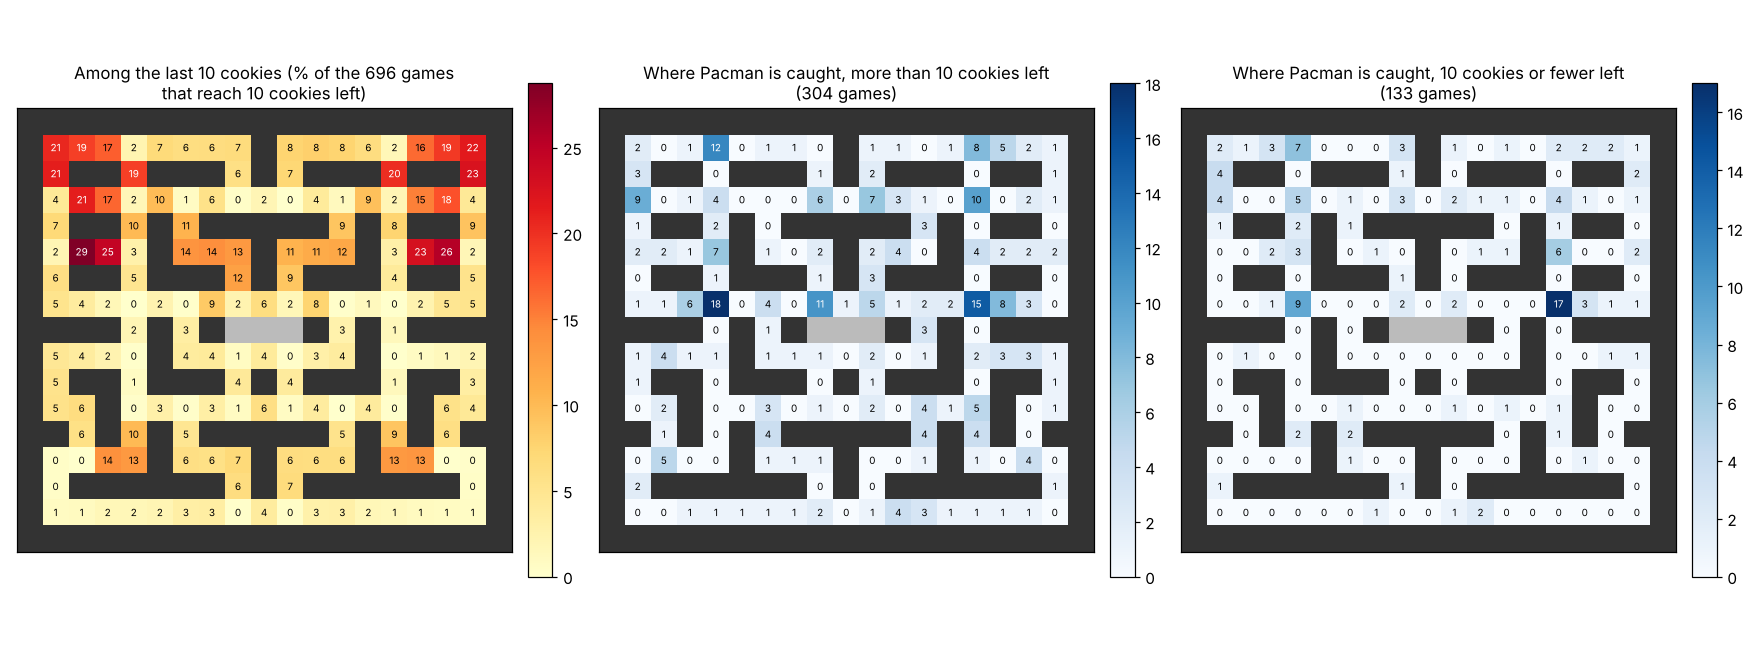
\includegraphics[width=\textwidth]{../Media/v2_endgame_heatmap.png}
  \caption{Run 1 on $1000$ games: how often each cell is among the last
    $10$ cookies (left), and where Pacman is caught, with more than $10$
    cookies left (middle) and with $10$ or fewer (right).}
  \label{fig:v2-heatmap}
\end{figure}

The heat map (\cref{fig:v2-heatmap}) shows where. The ghosts leave their
house by the door above it, into the corridor just above the house. Pacman
clears the bottom of the maze first and leaves the top corners for the end;
to reach them he must cross the junctions of that corridor, where the end
game is lost.

\begin{remark}{Lesson: find out how the agent loses}{lesson-diagnose}
  ``The agent is weak'' suggests nothing. ``The agent leaves the top
  corners for the end and is caught at their entrances'' suggests a cure.
  Each step of the diagnosis was a measurement on games the agent had
  already played: losses by stage, moves by distance to the ghosts, cells
  of the last cookies.
\end{remark}

\section{Practising the end of the game}

Two cures were considered. A larger reward for the cookies of the top
corners would push Pacman to eat them early, but it encodes the answer
(\emph{these} cells are dangerous) and suits this maze only. The other cure
changes only where some training games start.

\begin{definition}{Exploring starts}{exploring-starts}
  A method uses \emph{exploring starts} when its episodes do not all start
  from the initial state, but some start from other states, so that those
  states are visited often enough to be learnt. In Monte Carlo control,
  starting from every state--action pair with positive probability
  guarantees that every pair is evaluated.
\end{definition}

The \emph{late starts} of \code{run\_episodes} (option
\code{late\_start\_prob}) take their starting states from the agent's own
games: a game started from the beginning is copied (\code{env.clone()}) when
it reaches a number of cookies left drawn between $10$ and $40$, and a new
game starts from one of the last $2000$ copies with probability $0.25$. The
cookies left are where the agent's own play leaves them, the copies follow
the agent as it improves, and neither the rewards nor the rules change.

\begin{pacman}{Late starts}{late-starts}
  \emph{Run 3} resumed run 1 for $20$ million steps with late starts. The
  games that start late were won more and more often ($58\%$ to $64\%$),
  and on $3000$ new games run 3 wins $53.9\%$ of them: $3.8$ points more than
  run 1 ($3$ standard deviations of the difference) and $3.0$ more than
  run 2, which trained longer without late starts.
\end{pacman}

\begin{remark}{Lesson: prefer cures that do not encode the answer}%
  {lesson-neutral}
  A cure that only gives the agent more practice where it fails keeps the
  problem the same and adapts to the agent; a cure that tells the agent
  where the danger is solves one maze.
\end{remark}

\section{The rewards asked for the wrong thing}

Watching run 3 play showed something no statistic had: with power, Pacman
hunted the ghosts instead of clearing the maze. The rewards explain it. Two
rules of \code{v1} (\cref{tab:rewards}) were kept in \code{v2}: a cookie
eaten with power is worth nothing while a ghost is left in the game, so
that in \code{v1} the ghosts, which never come back, are hunted first; and
a power cookie is worth more when a ghost is close (\cref{eq:power-reward}).
In \code{v2} the eaten ghosts go back to the house, so a ghost is always
left: every cookie eaten with power was worth $0$, every ghost $5$, and the
power cookie paid for letting the ghosts come close. Pacman did what he was
paid for.

\begin{pacman}{New rewards}{new-rewards}
  In \code{v2} the cookies eaten with power now keep their reward $+0.8$,
  and a power cookie is worth a fixed $1.3$. \emph{Run 4}, trained from
  scratch with these rewards and the late starts for $60$ million steps on
  a Colab T4 ($19$ hours), wins its first games after $2$ million steps
  (run 1: $8$ million). On the same $3000$ new games, run 3 wins $54.5\%$ of
  them, run 4 $56.8\%$ after $50$ million steps (the budget of run 3) and
  $60.0\%$ after $60$ million.
\end{pacman}

\begin{remark}{Lesson: watch the agent, and read its rewards}{lesson-rewards}
  An agent optimises the rewards it is given, not the intention behind
  them. Rules that were right for one version of a problem can be wrong
  for the next. Watching games is a measurement too: it showed a
  behaviour that the win rates could not.
\end{remark}

\section{A flat curve, an improving agent}

\emph{Run 5} resumed run 4 at the final learning rate $2.5 \times 10^{-5}$
with the late starts. Its training games were won no more often (from
$52\%$ to about $54\%$), and the training was nearly stopped. Its
checkpoints said otherwise:
\begin{center}
  \begin{tabular}{@{}lc@{}}
    \toprule
    Same $3000$ games & Won \\
    \midrule
    run 4 ($60$ million steps) & $60.0\%$ \\
    run 5, $+5$ million & $60.5\%$ \\
    run 5, $+10$ million & $63.2\%$ \\
    run 5, $+15$ million & $64.5\%$ \\
    \bottomrule
  \end{tabular}
\end{center}
Since the best checkpoint was chosen on these games, it was evaluated again
on $3000$ others: $64.8\%$ (run 4: $59.9\%$).

The training games are played with sampled actions, and the policy's
entropy stayed at about $0.38$ nats: the sampled moves kept costing about
$10$ points of games won, while the best move kept improving. Run 2 had
shown the opposite: a rising training curve over an agent that did not
improve. In both cases the curve was the wrong measurement, which is the
lesson of \cref{rem:lesson-curve} again.

\section{How good can Pacman be?}

At $65\%$, is the agent good? Nothing so far said what a strong player could
do: with one life and three ghosts that never stop chasing, some games may
be lost whatever Pacman does. If the best possible play wins $70\%$, the
agent is excellent; if it wins $95\%$, the agent is the problem. A slow but
strong player answers: the open-loop MCTS of \cref{sec:mcts-v2}, with the
ghosts as chance, $100$ simulations per move near a ghost, and the agent as
prior and evaluator. On the same $100$ games it wins $82\%$ of them, against
$68\%$ for the agent alone, a significant difference
(\cref{pac:mcts-ceiling}). This player knows the ghosts' rules: its
simulations move them with the game's own code, though with random draws of
their own, not those of the real game. A fair player would have to estimate
the rules by watching the ghosts; on \code{v1}, the look-ahead search did as
well with such an estimate as with the exact rules (\cref{sec:ghost-models});
on \code{v2} it did not (\cref{sec:v2-fair}).

\begin{remark}{Lesson: measure the ceiling before investing}{lesson-ceiling}
  A strong but slow player tells whether the agent or the problem is the
  limit, and gives a target. Without it, more training could have been
  spent on a game whose ceiling was already reached; with it, the agent
  was known to be at least $15$ points short. State what the reference
  player knows: this one knew the ghosts' rules, which a fair player must
  estimate, and that turned out to be most of its advantage
  (\cref{sec:v2-fair}).
\end{remark}

\begin{remark}{Lesson: check a search against the agent alone}{lesson-check}
  The first version of the MCTS won $3$ of $20$ games that the agent alone
  won $14$ times: the value of a move did not include its own reward
  (\cref{rem:edge-reward}). A search that does worse than the network it
  uses is a bug until proven otherwise.
\end{remark}

\section{Teaching the network the search}

The search plays too slowly (about $8$ minutes per game on one core), so
expert iteration (\cref{sec:mcts-v2}) tries to move its skill into the
network: four iterations of $200$ games from run 5, with the visit
distributions of the MCTS as targets, $7.5$ hours on a Colab T4 with $8$ CPU
cores.

\begin{pacman}{Expert iteration on v2}{expert-v2}
  The search overrode the agent $9.6$ times per game at the first
  iteration, then $4.9$, $4.7$ and $4.3$: the network learnt about half of
  its corrections at once, then little more. On the $200$ games of each
  iteration the agent alone won $60\%$, $62\%$, $66.5\%$ and $67.5\%$, a
  rise that is within the noise ($3.4$ points per measurement). On the same
  $3000$ new games, compared game by game:
  \begin{center}
    \begin{tabular}{@{}lc@{}}
      \toprule
      Same $3000$ games & Won \\
      \midrule
      run 5 (start of the expert iteration) & $65.9\%$ \\
      after $4$ iterations & $67.3\%$ \\
      \bottomrule
    \end{tabular}
  \end{center}
  The expert agent wins $664$ games that the start agent loses and loses
  $624$ that it wins: under equal strength, a split at least as uneven has
  probability $0.28$ (two-sided, \cref{prop:sign-test}). The gain is at
  most small.
\end{pacman}

On \code{v1}, expert iteration recovered about $60\%$ of the search's gain
($97.1\%$ to $97.7\%$, the search reaching $98.1\%$,
\cref{pac:expert-results}); on \code{v2} about a tenth ($65.9\%$ to $67.3\%$,
the search reaching about $82\%$). The training statistics point to the
reason: the network reproduces only about $65\%$ of the search's
corrections on its own training data ($76\%$ on \code{v1}).

\begin{intuition}
  On \code{v2} the search adds \emph{computation}, not only knowledge.
  Before a dangerous move it simulates the ghosts' random moves dozens of
  times and finds an escape for this particular configuration of the
  three ghosts. A network has to turn that into a reflex, a fixed function
  of the screen, and it learns it from targets that are themselves noisy:
  with $100$ simulations the search does not always choose the same move in
  the same position. On \code{v1}, with fewer ghosts and a smaller maze,
  the search's corrections were simpler patterns, easier to learn.
\end{intuition}

A test separates the two explanations, noisy targets or a network too
small. On $300$ dangerous positions of the agent's own games, the search
was run twice, with different random numbers, with $100$ and with $400$
simulations. Two searches chose the same move on $97\%$ and $93\%$ of the
positions, but mostly because both followed the network: the search chose
the network's move on $92\%$ to $96\%$ of them. On the few positions where
it overrode the network, a second search made the same override only about
half the time ($6$ of $12$ with $100$ simulations, $9$ of $24$ with $400$).
The corrections that matter are close calls, decided by the random
simulations; a network cannot learn a coin flip, however large it is.

Several ways forward remain: a stronger and more consistent teacher (more
simulations), more data per iteration, a larger network; or keeping the PPO
training on the game's rewards with a penalty for straying from the search's
choices, as the KL penalty of RLHF keeps a policy close to a reference
(\cref{eq:rlhf-objective}), instead of pure imitation.

\section{Training longer}

The consistency test pointed to the simplest remaining lever: train longer
with the same network. \emph{Run 6} repeats run 4 (new rewards, late
starts, from scratch) over $100$ million steps instead of $60$, the learning
rate and the curriculum stretched over the longer training. It took $20$
hours on a Colab T4: a cache of the ghosts' shortest paths, written for the
search, made the game itself faster ($1400$ steps per second instead of
$870$). Its training curve rose steadily to the end; its checkpoints, on
the same $3000$ new games, tell a different story at the end.

\begin{pacman}{Training curve and agent}{run6}
  \begin{center}
    \begin{tabular}{@{}lccc@{}}
      \toprule
      Steps & Evaluation & Training & Gap \\
      \midrule
      $60$M & $52.6\%$ & $35.2\%$ & $17.4$ \\
      $80$M & $60.7\%$ & $43.8\%$ & $16.9$ \\
      $90$M & $63.4\%$ & $49.9\%$ & $13.5$ \\
      $100$M & $64.1\%$ & $55.0\%$ & $9.1$ \\
      \bottomrule
    \end{tabular}
  \end{center}
  Evaluation: best action, $3000$ new games. Training: games started from
  the beginning, around the checkpoint. From $60$ to $90$ million steps the
  agent improved by $11$ points; over the last $10$ million, the evaluation
  gained less than $1$ point and the training rate $5$. On the same games
  the expert agent wins $66.4\%$ of them: run 6 is not better
  ($p \approx 0.06$, \cref{prop:sign-test}).
\end{pacman}

\paragraph{Two kinds of randomness.} The ghosts are random in the training
games and in the evaluation alike. Pacman is random only in the training:
to explore, PPO samples its action from the policy, while the evaluation
plays the most probable action. If at each of $k$ dangerous moments of a
game the sampled action is a fatal one with probability $\varepsilon$, the
game survives these moments with probability $(1 - \varepsilon)^k$; with
$k = 20$ and $\varepsilon = 0.02$, that is $0.67$. As the policy becomes
more confident (its entropy fell from $0.50$ to $0.40$ nats), $\varepsilon$
decreases, and the training rate rises towards the evaluation even if the
best action does not change at all. The gap of the table shrinks for that
reason.

\begin{remark}{Lesson: a falling entropy lifts the training curve}%
  {lesson-entropy}
  The win rate of the training games mixes two things: how good the best
  action is, and how often the agent does not play it. A falling entropy
  alone makes the curve rise. Only the evaluation of the best action
  separates the two.
\end{remark}

Three different routes now end at the same level: fine-tuning ($75$ million
steps in all, $65.9\%$), expert iteration on top of it ($66$ to $67\%$), and a
longer schedule ($64.1\%$). When more training, more data and a teacher's
knowledge all stop at the same place, the limit is likely the agent itself:
a reflex that maps the last two images to a move, where surviving three
randomly moving ghosts sometimes needs looking a few moves ahead. The same
network wins $82\%$ of the games when it can look ahead
(\cref{pac:mcts-ceiling}).
Two directions follow: planning at play time, fairly, with a search that
estimates the ghosts' behaviour from their moves; or giving the network
more to work with, a memory (a recurrent network, more images) or a larger
field of view.

\section{A fair search}
\label{sec:v2-fair}

The first direction can be measured cheaply. A search whose ghosts follow a
generic model, with each ghost's two probabilities estimated from its moves
in the current game, is fair: it uses only what Pacman sees. It still knows
the form of the ghosts' behaviour, so it is an optimistic bound for any fair
planner, including one that would learn a model of the ghosts from scratch
(a world model). Before running it, a rule was fixed: if this search stays
near the agent's level, a learnt model would not be worth building.

It stayed there. On the same $60$ games, the run-6 agent won $71.7\%$ alone,
$66.7\%$ with the fair search and $80.0\%$ with the search knowing the rules
(\cref{pac:fair-mcts}); an earlier test with another agent gave the same
answer. Almost all of the search's gain came from knowing the ghosts'
rules, not from looking ahead. On this maze, the plateau of about $65\%$ is
close to what a fair player of this kind can reach.

The measurement itself went wrong once. The search had been made twice as
fast by running its simulations in waves (\cref{sec:mcts-v2}); a control
run with the same code as the fair search disagreed with the first
measurement made with the slower code, and the disagreement came from the
implementation. The question was then asked again, one simulation at a
time, on a machine with more cores.

\begin{remark}{Lesson: fix the stopping rule before the experiment}%
  {lesson-stopping}
  Deciding beforehand what result would stop a line of work (here: a fair
  search near the agent's level) lets the result decide, instead of being
  read to fit a plan. It also tells how precise the measurement must be:
  enough to tell $70\%$ from $80\%$, not more.
\end{remark}

\begin{remark}{Lesson: change one thing at a time, and control it}%
  {lesson-control}
  Two measurements made with two versions of the code differ by the
  question \emph{and} by the code. A control (the old question with the new
  code) separates the two; without it, a $10$-point effect of the
  implementation was nearly reported as an effect of the ghost model. And
  decide on the complete set of games: a difference that looked clear on
  $50$ games shrank on the next $20$.
\end{remark}

\section{The methods}

The agents of this chapter, each evaluated on $3000$ games that played no
part in its choice (the agent with the search on $100$ games):
\begin{center}
  \begin{tabular}{@{}lc@{}}
    \toprule
    Agent & Won \\
    \midrule
    run 1: PPO, curriculum, $30$M steps & $50\%$ \\
    run 3: late starts, $+20$M & $54\%$ \\
    run 4: new rewards and late starts, from scratch, $60$M & $60\%$ \\
    run 5: $+15$M at the final learning rate & $65\%$ \\
    expert iteration with the MCTS, $4$ iterations & $67\%$ \\
    run 6: as run 4, $100$M steps & $64\%$ \\
    \midrule
    agent with the MCTS (slow, knows the ghosts' rules) & $82\%$ \\
    agent with the MCTS, ghosts estimated (fair, $60$ games) & no gain \\
    \bottomrule
  \end{tabular}
\end{center}

Most of the progress came from understanding the problem, not from more
training: run 2's $35$ million extra steps brought nothing, while the
diagnosis of the losses and a second look at the rewards brought $15$
points. The methods, in the order they were needed:
\begin{enumerate}
  \item \textbf{Measure precisely}: thousands of games, standard errors
    (\cref{prop:win-rate-error}), and the agents compared game by game
    (\cref{prop:sign-test}).
  \item \textbf{Measure honestly}: the best of several agents confirmed on
    games that played no part in its choice (\cref{pac:lucky-games}).
  \item \textbf{Measure the agent, not the training}: the curve of the
    sampled policy can rise or stay flat whatever the agent does; a falling
    entropy alone lifts it.
  \item \textbf{Diagnose before curing}: when, where and how the games are
    lost (\cref{sec:v2-losses}).
  \item \textbf{Prefer neutral cures}: practise where the agent fails
    (exploring starts) rather than tell it the answer.
  \item \textbf{Watch the agent and read its rewards}: it optimises what it
    is paid for.
  \item \textbf{Estimate the ceiling}: a slow strong player says whether the
    agent or the problem is the limit.
  \item \textbf{Test the tools}: a search that loses to its own network is
    a bug.
  \item \textbf{Know what can be learnt}: a search's skill can be distilled
    into a network only as far as it is knowledge rather than computation,
    and its targets only as far as they are consistent.
  \item \textbf{Recognise a plateau}: when several independent routes stop
    at the same level, look at the agent's design, not at more training.
  \item \textbf{Measure fairly}: credit a search only with what a fair
    player could know; with the ghosts' rules estimated, the search's gain
    disappeared.
  \item \textbf{Control the code, fix the stopping rule}: compare a faster
    implementation with the slow one, and decide beforehand which result
    ends a line of work.
\end{enumerate}
